\section{MANIFOLDS}
\subsection{Topology}
A topology $\tau$ on a set X is a family of subsets of X, called
open sets, satisfying the following.

1. Arbitrary unions of open sets are open. \\
2. Finite intersections of open sets are open. \\
3. The empty set $\emptyset$ and X are both open.

A \textbf{topological space} (or simply a space) is a set X endowed with a topology.
Let X be a finite set and $\tau$ be the set of all subsets of X, then $\tau$ is called the \textbf{discrete topology} on X.
From the point of view of neighborhood, topology is also called the study of \textbf{nearness} relation.
\begin{figure}[ht]
    \begin{center}
        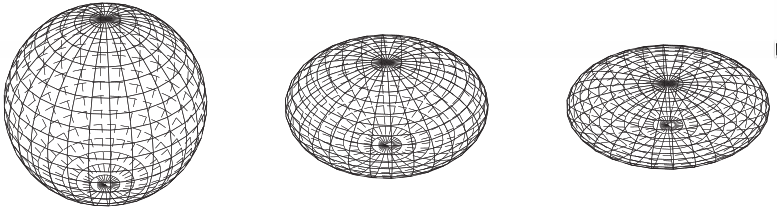
\includegraphics[width=\textwidth]{figures/topology_sphere.png}
        \caption{Topological 2-spheres}
    \end{center}
\end{figure}

All these shapes have the same topology but, since
the distance between the points on the surface has changed, they have different
geometries.

\subsection{Some Basic Set Terminologies}
\textbf{a. Open and Closed Sets:} A subset S of X is said to be an \textbf{open set} if every point of S is an interior point of S i.e.
\begin{center}
    $\forall$ x $\epsilon$ S $\exists \: \epsilon >$ 0 s.t. B(x; $\epsilon$) $\subset$ S.    
\end{center}
A subset S of X is called a \textbf{closed set} if $\overline{\text{S}}$ = X-S is open.

Some sets may be both open and closed, such sets are called \textbf{clopen sets}.

\textbf{b. Interior and Exterior: } Let S $\subset \mathbb{R}$ and x $\epsilon$ S then x is said to be an \textbf{interior point} of S if 
$\exists$ B(x; r) s.t. B(x; r) $\subset$ S. The set of all interior points of S is called the \textbf{interior} of S, \textbf{int(S)}.
Consequently, the union of all open sets contained in S is the int(S).

Similarly, x is called an \textbf{exterior point} of S if x is an interior point of X-S and the set of all exterior points of S
is called the \textbf{exterior} of S, \textbf{ext(S)}.

\textbf{c. Closure: } Closure of S $\subset$ X, \textbf{Cl(S)} is the intersections of all the closed sets cotaining S.
Set S is called \textbf{dense} if Cl(S) = X.

\textbf{d. Cover: } An \href{https://en.wikipedia.org/wiki/Cover_(topology)}{\textbf{open cover}} of S $\subset$ X is a collection of {U$_\alpha$} of open sets in X
whose union contains S i.e.
\begin{center}
    S $\subseteq$ U$_\alpha$
\end{center}
An open cover is \textbf{locally finite} if, for every x $\epsilon$ S , there is an open neighborhood B(x; r) of x
such that $\lvert$\{$\alpha$: U $\cap$ U$_\alpha$ $\neq \: \emptyset $\}$\rvert$ is finite. (Note that a locally finite open cover is not
necessarily finite.) An open cover {V$_\beta$ } is a \textbf{refinement} of {U$_\alpha$} if for all $\beta$ there is
an $\alpha$ such that U$_\alpha \supset$ V$_\beta$ .

\textbf{e. Compact: } A topological space X is \href{https://blogs.scientificamerican.com/roots-of-unity/what-does-compactness-really-mean/}{\textbf{compact}}
if every open cover has a finite subcollection that also covers X (“every open cover has a finite \textbf{subcover}”). 
Intuitively, compact spaces can be thought of as being finite in extent. 
For example, a subset of Euclidean space is compact if and only if it is closed and
bounded (\href{https://en.wikipedia.org/wiki/Heine%E2%80%93Borel_theorem}{\textbf{Heine-Borel theorem}}).

A \textbf{base/basis} for a topology $\tau$ of a topological space (X, $\tau$) is a family/collection, $\mathcal{B}$ of 
open sets of X s.t. every open set of the topology is equal to the union of some sub-family of $\mathcal{B}$ ($\mathcal{B}$ spans $\tau$).
Eg: the set of all open intervals in real number line $\mathbb{R}$ is a basis for Euclidean topology on $\mathbb{R}$ because every open
interval is an open set, and every open subset of $\mathbb{R}$ can be written as a union of some family of open intervals. The topology generated by $\mathcal{B}$ is just the collection of  open subsets of X where U is considered open
if $\forall$ x $\epsilon$ U $\exists$ B $\epsilon \: \mathcal{B}$ s.t. x $\epsilon$ B $\subset$ U.

Given two sets X and Y , the \textbf{product topology} on X $\times$ Y is the topology generated
by all sets of the form U $\times$ V, where U is open in X and V is open in Y. 
For Eg: The standard topology on $\mathbb{R}^n$ is the product topology on $\underbrace{\mathbb{R} \times ... \times \mathbb{R}}_{n \:times}$.

\subsection{Mapping Between Topologies}
Let f: X $\rightarrow$ Y be a map between topological spaces. The map f is \textbf{continuous}
if the inverse image of an open set S in Y is open in X.

Let $\tau$ be a topology on X, and let Y $\subset$ X. 
The collection $\tau_Y$ = {Y $\cap$ U: U $\epsilon \: \tau$} is a topology on Y, called the \textbf{induced topology} or \textbf{subspace topology} on Y. 
The space Y equipped with this topology is a \textbf{subspace} of X.

A map f: X $\rightarrow$ Y between topological spaces is a \textbf{homeomorphism} if it is
continuous with continuous inverse, meaning that there is a continuous map g: Y $\rightarrow$ X  such that g $\circ$ f = f $\circ$ g = 1. 
If such a pair of maps exist, we write X $\approx$ Y and say that X and Y are \textbf{homeomorphic} (or \textbf{topologically equivalent}). 
A \textbf{property} P(X) is a \textbf{topological invariant} of X if X $\approx$ Y implies P(X) = P(Y) i.e.
P(X) depends only on the topology of X. The property P(X) is a \textbf{complete topological invariant} of a space X provided that P(X) = P(Y) iff X $\approx$ Y. 
Topology can be loosely characterized as the study of the topological invariants of spaces.

\subsection{Multivariable Calculus} \label{Multivariable Calculus}
Let U $\subset \mathbb{R}^n$ be an open set and suppose that f: U $\rightarrow \mathbb{R}$ is a function. 
Label the points of $\mathbb{R}^n$ by the n-tuples x = (x$^1$, ..., x$^n$ ). Then the \href{https://en.wikipedia.org/wiki/Partial_derivative}{partial derivative} $\partial$f /$\partial$x$^i$
is defined by
\begin{equation}
    \frac{\partial f}{\partial x^i} = \lim_{h \rightarrow 0} \frac{f(x+he_i) - f(x)}{h}
\end{equation}

where e$_i$ = (0, ..., 1, ..., 0) has a “1” in the ith slot. For higher order, let $\alpha$ = (i$_1$, ..., i$_k$). Then
\begin{equation}
    \frac{\partial f}{\partial x^\alpha} (x) = \frac{\partial^k f}{\partial x^{i_1} ... \partial x^{i_k}}
\end{equation}

A function f: $\mathbb{R}^n$ $\rightarrow \mathbb{R}$ is \textbf{C$_\infty$}, or \href{https://en.wikipedia.org/wiki/Smoothness}{\textbf{smooth}}, 
if $\frac{\partial f}{\partial x^\alpha}$ exists and is continuous for
all $\alpha$. The composition of smooth functions is smooth.

Let U $\subset \mathbb{R}^n$ be an open set but now suppose that f: U $\rightarrow \mathbb{R}^m$ is a map,
given by x $\rightarrow$ (f$^1$(x), ..., f$^m$(x)). The map f is smooth if each component
function f$^1$ is smooth. The derivative D f(x) of f at x is just the matrix of partial
derivatives D f(x) = ($\partial f^i / \partial x^j$); this matrix is called the \href{https://en.wikipedia.org/wiki/Jacobian_matrix_and_determinant}{\textbf{Jacobian matrix}}.
When n = m, its determinant det($\partial f^i / \partial x^j$) is called the Jacobian determinant or more
simply the \textbf{Jacobian} of the map f.

Let U, V $\subset \mathbb{R}^n$ be two open sets, and let f: U $\rightarrow$ V be a homeomorphism.
If f and f$^{-1}$ are both smooth then f is called a \href{https://en.wikipedia.org/wiki/Diffeomorphism}{\textbf{diffeomorphism}} (isomorphism of smooth manifolds).
Since every diffeomorphism is a homeomorphism, given a pair of manifolds which are diffeomorphic to each other they are in particular homeomorphic to each other. 
The converse is not true in general. This brings us to the all-important \textbf{inverse function theorem (IFT)} which states, "if the matrix
representing the derivative of a function is invertible at some point then the function
itself is a \href{https://en.wikipedia.org/wiki/Local_diffeomorphism}{local diffeomorphism} in the neighborhood of that point".

\subsection{Coordinate Systems}
\href{https://en.wikipedia.org/wiki/N-sphere}{2-sphere}

Consider the transformation in $\mathbb{R}^2$ between Cartesian and polar coordinates:
\begin{equation}
    \begin{aligned}
        x = r cos\theta \\
        y = r sin \theta
    \end{aligned}
\end{equation}

Every point in the plane can be described uniquely in the (x, y) coordinate system,
but the \textbf{origin} is a problem for the polar coordinate system because it is described
by the infinity of pairs (r, $\theta$) = (0, anything). Another way to see that something
strange happens at the origin is to compute the Jacobian of the transformation.
\begin{equation}
    \begin{vmatrix}
        \partial x / \partial r & \partial x / \partial \theta \\ 
        \partial y / \partial r & \partial y / \partial \theta 
   \end{vmatrix} = 
   \begin{vmatrix}
    cos \theta & -r sin \theta \\ 
    sin \theta & r cos \theta 
\end{vmatrix} = r
\end{equation}

Now, at origin r vanishes and consistently the Jacobian determinant.

The \textbf{IFT} provides the link between these two ways of
determining the validity of a given coordinate transformation. A coordinate transformation is a good one 
if there is a one-to-one correspondence between the two sets of coordinates and if the transformation is differentiable.
In other words, a set of functions {f$^i$(x)} on $\mathbb{R}^n$ constitutes a \textbf{good coordinate system} in the 
neighborhood of a point x if the transformation (x$^1$, ..., x$^n$ ) $\rightarrow$ (f$^1$ (x$^1$, ..., x$^n$ ), ..., f$^n$ (x$^1$, ..., x$^n$)) is a diffeomorphism.
Ascertaining whether a map is a diffeomorphism can be difficult. 
But checking whether a Jacobian vanishes is usually easy. 
The \textbf{IFT} assures that, as long as the Jacobian of the transformation is nonsingular, 
we can coordinatize the neighborhood of x with the functions f$^i$.

\subsection{Differential Manifold (Smooth Manifold or C\texorpdfstring{$_\infty$ } d)}
An n-dimensional smooth manifold \textbf{M} consists of a  \href{https://en.wikipedia.org/wiki/Hausdorff_space}{\textbf{Hausdorff} topological space}
together with a \textbf{countable} collection of open sets \{U$_i$\}, called \textbf{coordinate neighborhoods/patches}, 
that \textbf{cover} \textbf{M} and a collection of maps \{$\psi_i$\}, called \textbf{coordinate
maps}, satisfying two conditions.

1. Each $\psi_i$: U $\rightarrow \mathbb{R}^n$ is a homeomorphism onto an open subset of Rn . (We say
that \textbf{M} is \textbf{locally Euclidean}.) \\
2. If U$_i$ and U$_j$ are two overlapping coordinate neighborhoods with coordinate maps $\psi_i$ and $\psi_j$ 
then $\psi_j \circ$ $\psi_i^{-1}$: $\psi_i$ (U$_i$ $\cap$ U$_j$) $\rightarrow \psi_j$ (U$_i$ $\cap$ U$_j$) is
a diffeomorphism. (We say that the coordinate maps are \textbf{compatible} on
overlaps.)

Each pair (U$_i$ , $\psi_i$) is called a \textbf{coordinate chart}, and the collection of all coordinate
charts is called an \textbf{atlas}. The maps $\psi_j \circ$  $\psi_i^{-1}$ are called \textbf{transition functions} of the
atlas.

The \href{https://www.quora.com/What-is-the-significance-of-Hausdorff-Spaces-How-do-these-measurements-help-us-What-does-it-allow-us-to-have}{\textbf{Hausdorff condition}}
is there basically to express our intuition of space as “infinitely divisible”, so that we can separate points with open sets. 
The condition that the \textbf{cover be countable} is there for a technical reason having to do
with extending locally defined quantities to globally defined ones. 
The condition that \textbf{M} be \textbf{locally Euclidean} serves at least two purposes. 
First, it tells us that, in the neighborhood of a point, all n-dimensional manifolds look like a (mildly deformed) bit of Euclidean n-space. 
Second, it allows us to define local coordinates so that we can compute things. 
The compatibility condition ensures that we can patch together the coordinate systems consistently, so that we always end up with valid coordinates.
\begin{figure}
    \begin{center}
        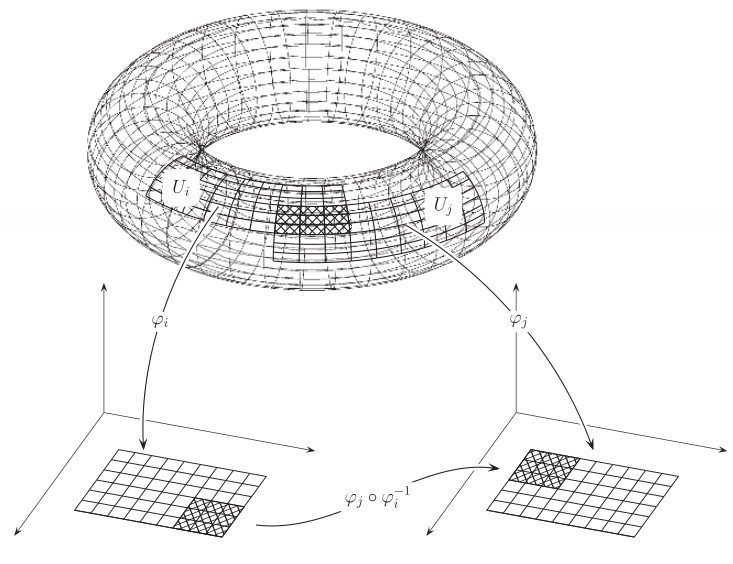
\includegraphics[width=0.75\textwidth]{figures/coordinate-chart.png}
        \caption{Two coordinate charts and a transition function}
    \end{center}
\end{figure}

Let (U, $\psi$) be a coordinate chart with p $\epsilon$ U and suppose that $\psi$(p) = q. If
x$^1$ , . . . , x$^n$ are the standard coordinate functions on $\mathbb{R}^n$ then q has coordinates
(x$^1$(q), . . . , x$^n$(q)). Thus we can write
\begin{equation}
    \psi(p) = (x^1(q), . . . , x^n(q))
\end{equation}

The functions x$^1$ , . . . , x$^n$, viewed as functions on U , are called \textbf{local coordinates} on U. 
Let V be another coordinate neighborhood, with local coordinates y$^1$ , . . . , y$^n$. 
If U$\cap$V = $\phi$ then on $\psi$(U$\cap$V) the action of the transition function $\psi_1 \circ$  $\psi_2^{-1}$ can be
written in local coordinates as follows:
\begin{equation}
    (x^1 , . . . , x^n ) \rightarrow (y^1 (x^1 , . . . , x^n ), . . . , y^n (x^1 , . . . , x^n ))
    \label{eqn:local_coord}
\end{equation}

The compatibility condition (2) in the definition of a manifold is just the statement that equation \ref{eqn:local_coord} is a diffeomorphism, which, by the inverse
function theorem, is equivalent to the requirement that the Jacobian determinant
det($\partial$y$_i$/$\partial$x$_j$) be nonzero. The sign of this determinant is important. 
A manifold is said to be \href{https://en.wikipedia.org/wiki/Orientability}{\textbf{orientable}}
if it is possible to choose an ordering of the local coordinates so that the Jacobian
determinants of the transition functions have the same sign on every pair of overlapping neighborhoods. 
If this is possible then the manifold has two opposite orientations, according to the choice of sign.

\subsection{Smooth Maps on Manifolds}
The definition of the derivative given in Section \ref{Multivariable Calculus} uses the linear structure of
Euclidean space in a crucial way, and there is no way to define something similar
for a general curved space. Instead, the existence of the coordinate maps on
a smooth manifold is used to define differentiability.

A function f: \textbf{M} $\rightarrow \mathbb{R}$ is smooth at p $\epsilon$ \textbf{M} if, for any chart (U, $\psi$)
with p $\epsilon$ U, the map
\begin{equation}
    \widetilde{f}= f \circ \psi^{-1}:\psi(U) \rightarrow \mathbb{R}
\end{equation}

is a smooth function in the usual Euclidean sense near $\psi$(p).

In general, Let \textbf{M} and \textbf{N} be two smooth manifolds of dimensions m and n, respectively. 
A map f: \textbf{M} $\rightarrow$ \textbf{N} is smooth if $\forall$ p $\epsilon$ \textbf{M} $\exists$ charts (U, $\psi_1$) on \textbf{M} and (V, $\psi_2$) on \textbf{N}, 
with p $\epsilon$ U and f(U) $\subset$ V s.t.
\begin{equation}
    \widetilde{f}= \psi_2 \circ f \circ \psi_1^{-1}:\psi_1(U) \rightarrow \psi_2(V)
\end{equation}

is a smooth map of Euclidean spaces. A smooth map f: \textbf{M} $\rightarrow$ \textbf{N} is a \textbf{diffeomorphism} 
if f$^{-1}$ exists and is smooth, in which case we say that \textbf{M} and \textbf{N} are diffeomorphic.

Because smooth maps of manifolds reduce to smooth maps of Euclidean space, 
the inverse function theorem works for manifolds in the same way as it does in Euclidean space: 
if the Jacobian matrix of f is nonsingular then f is a local diffeomorphism. 
In particular, M and N can only be \textbf{diffeomorphic} if m = n.

\subsection{\href{https://mathweb.ucsd.edu/~eizadi/250A-2019/Patrick-Girardet.pdf}{Immersion and Embedding}}
A prototypical theme in geometry is the study of “\textbf{spaces with structure}”, i.e.
a set X equipped with some sort of additional geometric structure, such as a
topology in the case of topological spaces. It is important how
functions between our spaces with structure interact with the structure on those
spaces. We concern ourselves only with those functions which “preserve” the
structure (e.g. \textbf{differentiable maps} between {differentiable manifolds}, 
which are maps respecting the differentiable structure).

A differentiable mapping f: \textbf{M}$^m \rightarrow$ \textbf{N}$^n$ (m = dim \textbf{M}, n = dim \textbf{N})
of differentiable manifolds \textbf{M} and \textbf{N} is said to be an \href{https://en.wikipedia.org/wiki/Immersion_(mathematics)}{immersion}
if df$_p$: T$_p$\textbf{M} $\rightarrow$ T$_{f(p)}$\textbf{N} is injective $\forall$ p $\epsilon$ \textbf{M} where
T$_p$\textbf{X} denotes the \textbf{tangent space} [\ref{Tangent Space}] of manifold \textbf{X} at point p $\epsilon$ \textbf{X}.

Equivalently, f is an immersion if its derivative \textbf{df} has a constant rank = m i.e. rank(df) = dim \textbf{M} = m.
The function itself need not be injective, only its derivative \textbf{df} must be.

Since df: T$_p$\textbf{M} $\rightarrow$ T$_{f(p)}$\textbf{N} is a linear map between vector spaces
and dim T$_p$\textbf{M} = dim \textbf{M} = m $\forall$ p $\epsilon$ \textbf{M}, 
it follows by linear algebra that if df is an immersion then dim \textbf{M} $\leq$ dim \textbf{N}. 
We call dim \textbf{N} - dim \textbf{M} the \textbf{codimension} of df.
\begin{figure}[ht]
    \begin{center}
        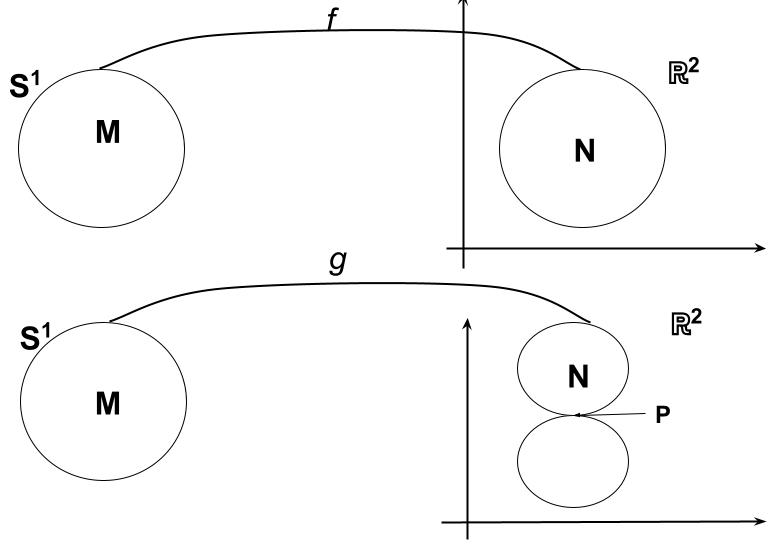
\includegraphics[width=0.5\textwidth]{figures/embedding-immersion.png}
        \caption{\textit{f} is an immersion as well as embedding but \textit{g} is only immersion due to self-intersection at p, which doesn't allow homeomorphism.}
    \end{center}
\end{figure}

If f is an immersion $\forall$ p $\epsilon$ \textbf{M} then \textbf{M} is an (immersed) \textbf{submanifold} of \textbf{N}.
The Jacobian has \textbf{maximal rank} (namely m), so f(M) is locally coordinatizable according to the IFT. 
If m $\geq$ n and the Jacobian of the transformation has maximal rank (namely n) at p $\epsilon$ \textbf{M} then f is called a
\textbf{submersion} at p.

An injective immersion f is called an \textbf{embedding} provided
that f maps \textbf{M} homeomorphically onto its image f(\textbf{M}) (in the induced topology). 
The basic difference between immersions and embeddings is that the image
of an immersion can have \href{https://en.wikipedia.org/wiki/List_of_self-intersecting_polygons}{\textbf{self-intersections}} 
whereas the image of an embedding cannot. 

The \href{https://en.wikipedia.org/wiki/Whitney_embedding_theorem}{\textbf{Whitney embedding theorem}} says that
any n-dimensional topological manifold can be embedded in $\mathbb{R}^{2n+1}$, and any n-dimensional smooth manifold can be embedded in $\mathbb{R}^{2n}$.
The  Möbius strip is a smooth 1-manifold and can be embedded in $\mathbb{R}^{3}$ and 
the Klein bottle is a smooth 2-manifold and thus can be embedded in $\mathbb{R}^{4}$. 
If you try to construct the Klein bottle in $\mathbb{R}^{3}$, 
you will observe that you cannot do it without creating self-intersections somewhere.
Whitney's result means that, without loss of generality, we could simply treat
manifolds as living in a large Euclidean space. The intrinsic description of a manifold also has physical utility. Einstein modeled
the universe as a smooth manifold of a certain type.

\begin{figure}[ht]
    \begin{center}
        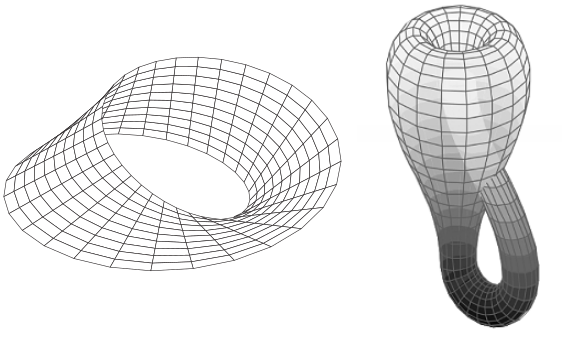
\includegraphics[width=0.5\textwidth]{figures/moebius-klien.png}
        \caption{Möbius strip immersed in $\mathbb{R}^{2}$ (left) and Klein bottle immersed in $\mathbb{R}^{3}$ (right)}
    \end{center}
\end{figure}

\subsection{Tangent Space}\label{Tangent Space}
The \href{https://en.wikipedia.org/wiki/Tangent_space}{\textbf{tangent space}} is a space spanned by
the tangent vectors of curves lying in that space. The tangent space of a manifold generalizes to higher dimensions 
the notion of tangent planes to surfaces in 3D and tangent lines to curves in 2D. 
In the context of physics the tangent space to a manifold at a point can be viewed as the space of possible velocities 
for a particle moving on the manifold ($\overrightarrow{v}$ = $\partial \overrightarrow{r}/ \partial t$).

Once the tangent spaces of a manifold have been introduced, one can define vector fields, which are abstractions of the velocity field of particles moving in space. 
A vector field attaches to every point of the manifold a vector from the tangent space at that point, in a smooth manner. 
Such a vector field serves to define a generalized ordinary differential equation on a manifold: 
A solution to such a differential equation is a differentiable curve on the manifold whose derivative at any point is equal to the 
tangent vector attached to that point by the vector field. 
All the tangent spaces of a manifold can be glued together to form a new differentiable manifold
with twice the dimension of the original manifold, called the \href{https://en.wikipedia.org/wiki/Tangent_bundle}{\textbf{tangent bundle}}
of the manifold.

Let us define a tangent vector X$_p$ at a point p $\epsilon$ \textbf{M} to be a \textbf{linear derivation} at p. 
This means that, $\forall$ a, b $\epsilon$ $\mathbb{F}$ and
f, g $\epsilon$ $\Omega^0$(\textbf{M}), X$_p$ : $\Omega^0$(\textbf{M}) $\rightarrow \mathbb{R}$ satisfies

1. \textbf{linearity}: X$_p$ (af + bg) = a X$_p$ (f) + bX$_p$ (g), and \\
2. \textbf{Leibniz property}: X$_p$ (f g) = g(p)X$_p$ (f) + f (p)X$_p$ (g).

The vector space T$_p$\textbf{M} generated by all the X$_p$ is called the \textbf{tangent space to
M at p}. It is important to note that the tangent space T$_p$\textbf{M} is defined independently of any
coordinate system. Thus, at each point we are free to pick any basis \{e$_i$\}, not just
a coordinate basis \{$\partial$/$\partial$ x$_i$\}. Any smoothly varying basis on \textbf{M} is called a \textbf{frame field}.
Generally, frame fields do not exist everywhere on \textbf{M}; they clearly exist
locally, because e$_i$ = $\partial$/$\partial$ x$_i$  is an instance. In terms of a frame field \{e$_i$\}, we could
write a vector field X as
\begin{equation}
    X = X_i e_i
\end{equation}

\begin{figure}[ht]
    \begin{center}
        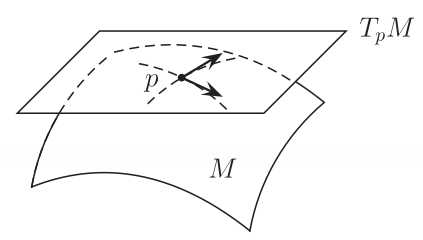
\includegraphics[width=0.5\textwidth]{figures/tangent-space.png}
        \caption{Although the tangent space T$_p$\textbf{M} is an abstract linear space attached to
        \textbf{M} at p, we often imagine it to look like above figure.}
    \end{center}
\end{figure}

\subsection{Cotangent Space}
The cotangent space $T_{p}^{*}$\textbf{M} is defined as the dual space of the tangent space at p, 
$T_{p}$\textbf{M}. The elements of the cotangent space are called \textbf{cotangent vectors} or \textbf{tangent covectors}.
All cotangent spaces at points on a connected manifold have the same dimension, equal to the dimension of the manifold. 
All the cotangent spaces of a manifold can be "glued together" (i.e. unioned and endowed with a topology) to form a new differentiable manifold of twice the dimension, the cotangent bundle of the manifold.

Let  \textbf{M} be a smooth manifold and let  p be a point in \textbf{M}. 
Let  $T_{p}$\textbf{M} be the tangent space at p. 
Then the cotangent space at p is defined as the dual space of $T_{p}$\textbf{M}:
\begin{equation}
    T_{p}^{*}\textbf{M} = (T_{p}\textbf{M})^{*}
\end{equation}
Concretely, elements of the cotangent space are \textbf{linear functionals} on 
$T_{p}$\textbf{M} i.e. every element $\alpha \: \epsilon \: T_p$\textbf{M} is a linear map
$\alpha$ :$T_{p}$\textbf{M} $\rightarrow \mathbb{F}$

where $\mathbb{F}$ is the underlying field of the vector space being considered, for example, the field of real numbers. 
The elements of $T_{p}^{*}$\textbf{M} are called cotangent vectors.

Let \{x$^i$\} be local coordinates  around p, then T$_p$\textbf{M} is spanned by the n basis vectors $\partial/\partial x^i$. The
corresponding dual basis vectors are denoted dx$^i$. By definition we have
\begin{equation}
    \Bigg< \frac{\partial}{\partial x_i}, dx^j\Bigg> = \delta_i^j
\end{equation}

A general element $\alpha$ p of T$_p^*$\textbf{M} is a linear combination of
the basis elements:
\begin{equation}
    \alpha_p = a_i dx^i
\end{equation}
where $\alpha_i$ are constants.

A \textbf{differential} \href{https://mathworld.wolfram.com/One-Form.html}{\textbf{1-form}} or \textbf{smooth covector field}
on \textbf{M} is a smooth map p$\rightarrow \alpha_p$. In local coordinates around p 
\begin{equation}
    \alpha = a_i(x)dx^i
\end{equation}
where the a$_i$(x) are smooth functions on \textbf{M}.

\textbf{1-forms} (covector/pseudovector) of a vector space with local coordinates (dx$_1$, dx$_2$, ..., dx$_n$)
are the elements of a vector space with local basis (dx$^1$, dx$^2$, ..., dx$^n$) i.e. dual space.
(Vectors (covariant vectors/\textbf{kets} $|\psi \rangle$) and 1-forms (contravariant vectors/\textbf{bras} $\langle \psi |$) are dual to each other.)
\textbf{2-forms} are the elements of the exterior product space with local basis (dx$^1 \exterior$ dx$^2$, dx$^2 \exterior$ dx$^3$ ..., dx$^{n-1} \exterior$ dx$^n$).
In general, (\href{https://www.physicsforums.com/threads/what-is-2-form.762846/#:~:text=The%201%2Dforms%20(or%20covectors,the%20bases%20may%20be%20omitted.}{\textbf{k-form}})
(or a form of degree k) are the elements of the exterior product space with basis (dx$^1 \exterior$ dx$^2 ... dx^p$, ...). For eg:
in 3D Euclidean space with basis (i, j, k), 

1-form have basis (i', j', k') \\
2-form have basis (j$\exterior$k, k$\exterior$i, i$\exterior$j) \\
3-form have basis (i$\exterior$j$\exterior$k) \\
other higher forms don't exist for 3D.

Like tangent space, cotangent space is also independent of any particular coordinate system for its definition. 
If \{e$_i$\} is a generic basis for T$_p$\textbf{M} then the corresponding dual basis \{$\theta^i$\} is called a \textbf{coframe field}, so
\begin{equation}
    \Big<e_i, \theta^j\Big> = \delta_i^j
\end{equation}

\subsection{Cotangent Space as \href{https://en.wikipedia.org/wiki/Jet_(mathematics)}{Jet Space} }
We have defined a differential 1-form as a smoothly varying map
on M that assigns to every point p of M an element of the cotangent space at p.
Although this is correct, it is perhaps rather unsatisfying because the cotangent
space is defined in terms of the tangent space, which is itself defined as a space of
derivations on functions. There is, however, an elegant way to define the cotangent
space directly, using just the notion of a smooth function, which is perhaps a bit
more natural from the point of view of manifold theory. It uses the idea of a \textbf{jet}.
Jet is an operation that takes a differential function \textit{f} and produces a polynomial,
the truncated Taylor polynomial of \textit{f} at each point of its domain. 
The theory of jets regards these polynomials as abstract polynomials rather than polynomial functions.
\begin{equation}
    (J_{x_0}^k f)(z) = \sum_{i=0}^{k} \frac{f^{(i)}(x_0)}{i!}z^i = f(x_0) + f'(x_0)z + ... + \frac{f^{(k)}(x_0)}{k!}z^k
\end{equation}
gives the k-jet of f:$\mathbb{R} \rightarrow \mathbb{R}$ at point x$_0$ in 1D case.

Let C$^\infty$($\mathbb{R}^n, \mathbb{R}^m$) be a vector space of smooth functions f:$\mathbb{R}^n \rightarrow \mathbb{R}^m$.
Let k is a non-negative integer and p $\epsilon \mathbb{R}^n$, then we can define an equivalence relation \textbf{E}$^k_p$ on C$^\infty$
by declaring that two functions \textit{f} and \textit{g} are equivalent to the order of k if they have the same value at p,
and all their partial derivatives agree at p upto their kth derivatives i.e.
\textit{f} $\sim$ \textit{g} iff \textit{f}-\textit{g} = 0 to kth order.
The \textbf{kth order jet space} of C$^\infty$($\mathbb{R}^n, \mathbb{R}^m$) at p is defined as the set of 
equivalence classes of \textbf{E}$^k_p$ and is denoted by J$^k_p$($\mathbb{R}^n, \mathbb{R}^m$).

Now, let \textit{f}:\textbf{M} $\rightarrow \mathbb{R}$ be a smooth function, p$\epsilon$\textbf{M}, and \{x$^i$\} local coordinates around
p. We say that \textit{f} vanishes to first order at p if $\partial f /\partial x^i$ vanishes at p for all i.
for k$\geq$1 we say that \textit{f} vanishes to kth order at p if, $\forall$ i, $\partial f /\partial x^i$ vanishes to (k-1)th order at p,
where \textit{f} vanishes to zeroth order at p if \textit{f}(p) = 0. 
In other words, \textit{f} vanishes to kth order at p if the first k terms in its Taylor expansion vanish at p.

For k$>$0 let \textbf{M}$^k_p$ be the set of all smooth functions on \textbf{M} vanishing to (k-1)th order at p, 
and set \textbf{M}$^0_p$:= $\Omega^0$(\textbf{M}) and M$_p$ := \textbf{M}$^1_p$. Each \textbf{M}$^k_p$ is a vector
space under the usual pointwise operations, and we have the series of inclusions
\begin{center}
    \textbf{M}$^0_p \supset$ \textbf{M}$^1_p \supset$ \textbf{M}$^2_p \supset$ ....    
\end{center}

We now define T$_p^*$\textbf{M}, the cotangent space to \textbf{M} at p, to be the
\href{https://www.youtube.com/watch?v=nh-YgZph-r4}{\textbf{quotient space}} 
\begin{equation}
    T_p^*\textbf{M} = \textbf{M}_p/\textbf{M}^2_p
\end{equation}
An element of T$_p^*$\textbf{M} is called a \textbf{differential 1-form} at p.

\subsection{Tensor Field}
There are many different ways to define a tensor field on a manifold, but the essential idea is simple enough: 
just like a vector field is an assignment of vectors to each point in space (manifold \textbf{M}), a tensor field is just a smooth assignment of a tensor to every point of \textbf{M}.  
A tensor field $\Psi$ of type (r, s) can also be defined as a map from \textbf{M} to \textbf{T}$^s_r$ s.t. on any coordinate
patch U, the components $\Psi^{i_1 i_2...i_r}_{j_1 j_2...j_s}$ are smoothly varying functions. 
\begin{equation}
    \Psi = \Psi^{i_1 i_2...i_r}_{j_1 j_2...j_s} \frac{\partial}{\partial x^{i_1}} \otimes ... \otimes \frac{\partial}{\partial x^{i_r}} \otimes dx^{j_1} \otimes ... \otimes dx^{j_s}
\end{equation}

where for any p $\epsilon$ U , the vector fields $\frac{\partial}{\partial x^{i_i}}$ and the 1-form fields dx$^i$ constitute dual bases for
T$_p$\textbf{M} and T$_p^*$\textbf{M} respectively, thus forming a basis of tensor product space (T$_p$\textbf{M})$^{\otimes r} \otimes$ (T$_p^*$\textbf{M})$^{\otimes s}$.

\begin{figure}[ht]
    \begin{center}
        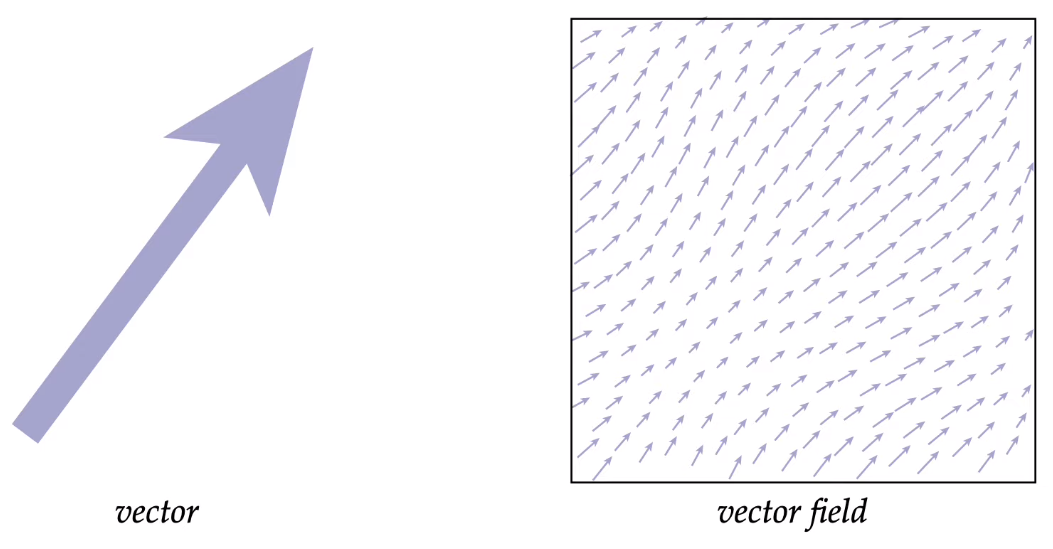
\includegraphics[width=0.5\textwidth]{figures/vector_field.png}
        \caption{Just like a vector field is an assignment of vectors to each point in space (manifold),
        a tensor field is an assignment of tensors to each point in space (manifold)}
    \end{center}
\end{figure} 

Tensor field can also be viewed as a smoothly varying multilinear map. 
Let $\widetilde{\textbf{T}}^s_r$(p) be the space of all multilinear maps on (T$_p^*$\textbf{M})$^{\times r} \times$ (T$_p$\textbf{M})$^{\times s}$.
A tensor field $\Psi$ of type (r, s) is then a smooth assignment of an element $\Psi_p \: \epsilon$
$\widetilde{\textbf{T}}^s_r$(p) to each p $\epsilon$ \textbf{M}. 
The map $\Psi$ must be more than just multilinear-in fact, it must be \href{https://math.stackexchange.com/questions/2138459/understanding-the-definition-of-tensors-as-multilinear-maps}{functional multilinear}, 
which means that equation \ref{eqn:functional_multilinear} must hold for $\Psi$.
\begin{equation}
    \Psi(v_1, ..., \alpha_1 u + \alpha_2 w, ..., v_{r+s}) = \alpha_1 \Psi(v_1, ..., u, ..., v_{r+s}) + \alpha_2 \Psi(v_1, ..., w, ..., v_{r+s})
    \label{eqn:functional_multilinear}
\end{equation}
where $\alpha_1$ and $\alpha_2$ are smooth functions on \textbf{M}. And thus,
\begin{equation}
    \Psi: \underbrace{\Gamma(T^*\textbf{M}) \times ... \times \Gamma(T^*\textbf{M})}_{r \:times} \times \underbrace{\Gamma(T \textbf{M}) \times ... \times \Gamma(T \textbf{M})}_{s\: times} \rightarrow \Omega^0 (\textbf{M})
    \label{eqn:0-form}
\end{equation}
where $\Gamma$(T \textbf{M}) and $\Gamma$(T$^*$ \textbf{M}) denote the space of all vectors and covectors fields on \textbf{M}.

\subsection{Differential Forms}
Just as a k-vector is a special kind of tensor (\href{https://web2.clarkson.edu/projects/subramanian/ch490/notes/Alternating%20Unit%20Tensor.pdf}{alternating tensor}), a k-form is a
special kind of tensor field (alternating tensor field).  
k-forms are by far the most useful kind of tensor fields, for several reasons:

1.They are easy to define. \\
2. They are easy to use because, for the most part, one does not have to deal with all those irritating indices. \\
3. Almost all important geometrical quantities can be expressed in terms of forms. \\
4. Differential forms are essentially the things that appear under integral signs.

Let U be a coordinate patch of \textbf{M} and let p $\epsilon$ U. A k-form $\omega_p$ on U at p is an element of k (T$_p^*$\textbf{M}). 
It follows that, in local coordinates,
\begin{equation}
    \omega_p = \frac{1}{k!}\sum a_{i_1...i_k}dx^{i_1}\exterior...\exterior dx^{i_k} = \sum a_I dx^I
\end{equation}

for some constants a$_I$ = a$_{i_1...i_k}$. A (differential) k-form $\omega$ on \textbf{M} is a smooth
assignment p $\rightarrow \omega_p$. In local coordinates,
\begin{equation}
    \omega_U = \frac{1}{k!}\sum a_{i_1...i_k}(x)dx^{i_1}\exterior...\exterior dx^{i_k} = \sum a_I(x) dx^I
\end{equation}

where the a$_I$(x) are now smooth functions on U. 
The vector space of all k-forms on \textbf{M} is denoted $\Omega^k$(\textbf{M}). 
In particular, we think of the smooth functions on \textbf{M} as \textbf{0-forms} as shown in equation \ref{eqn:0-form}.

\begin{figure}[ht]
    \begin{center}
        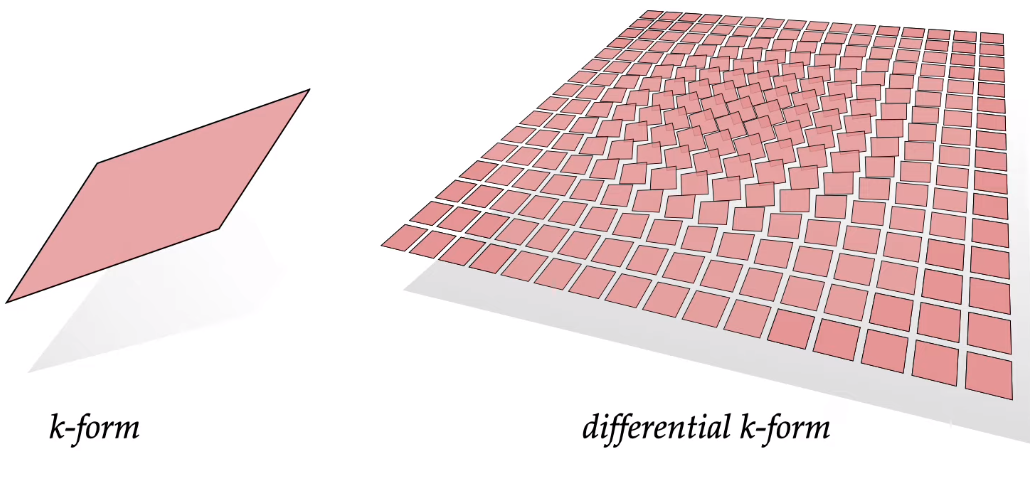
\includegraphics[width=0.5\textwidth]{figures/differential_k-form.png}
        \caption{Just like a vector field is an assignment of vectors to each point in space (manifold), 
        a differential k-form is an assignment of k-forms to each point in space (manifold)}
    \end{center}
\end{figure}

\subsection{Exterior Derivative}
We now introduce a natural differential operator on k-forms, denoted by 'd'. 
It is a far reaching generalization of the ordinary gradient, curl, and divergence operators of multivariable calculus.

\textbf{Theorem: } There exists a unique linear operator d:$\Omega^k$(\textbf{M}) $\rightarrow$ $\Omega^{k+1}$(\textbf{M}) called the exterior derivative, satisfying the following properties. 
For any forms $\lambda$ and $\mu$, and for any function \textit{f} , the operator d is

1. \textbf{linear:} d($\lambda$ + $\mu$) = d$\lambda$ + d$\mu$,\\
2. \textbf{graded derivation:} d($\lambda \exterior \mu$) = d$\lambda \exterior \mu$ + (-1)$^{(deg \lambda)} \lambda \exterior$ d$\mu$,\\
3. \textbf{nilpotent:} d$^2 \lambda$ = 0, and \\
4. \textbf{natural:} in local coordinates \{x$_i$\} about a point p, d\textit{f} = $\sum \frac{\partial \textit{f}}{\partial x^i} dx^i$.

\subsection{Interior Product (Interior Derivative)}
Interior product is a degree -1 (anti)derivation on the exterior algebra of differential forms on a smooth manifold.
Given a vector field X we can define a linear map i$_X$ : $\Omega^k$(\textbf{M}) $\rightarrow \Omega^{k-1}$ (\textbf{M}), taking
k-forms to (k-1)-forms, called the interior product, satisfying the following
properties. Let f be a function, $\omega$ a 1-form, and $\lambda$ and $\eta$ arbitrary-degree forms. Then

1. i$_X$f = 0 \\
2. i$_X \omega$ = $\omega$(X) := $\langle \omega, X \rangle$ \\
3. \textbf{graded derivation:} i$_X$($\lambda \exterior \eta$) = i$_X \lambda \: \exterior \eta$ + (-1)$^{deg \lambda} \lambda \: \exterior$ i$_X \eta$.

\subsection{Pullback and Pushforward}
Let \textit{f}: \textbf{M}$\rightarrow$\textbf{N} be a smooth map of manifolds.  
Given a smooth map \textit{g}: \textbf{N}$\rightarrow \mathbb{R}$ we define a new map $f^*g$: \textbf{M}$\rightarrow \mathbb{R}$ by  $f^*g$ = $g\circ f$. 
The map $f^*g$ is called the \textbf{pullback} of \textit{g} by \textit{f}, because the function \textit{g} is “pulled back” from \textbf{N} to \textbf{M}.
In simple terms, pullback is the composition of smooth maps. 
Apullback map is extended to forms by requiring it to be

1. \textbf{a ring homomorphism: } $f^*(\lambda + \mu)$ = $f^*\lambda$ + $f^*\mu$, $f^*(\lambda \exterior \mu)$ = $f^*\lambda \exterior f^*\mu$ and \\
2. \textbf{natural: } d($f^*\lambda$) = $f^*$(d$\lambda$).

\begin{figure}[ht]
    \begin{center}
        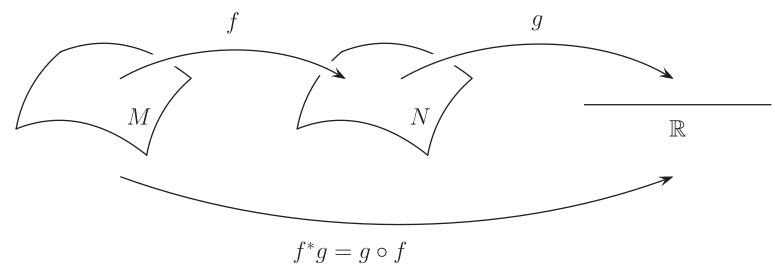
\includegraphics[width=0.5\textwidth]{figures/pullback.png}
        \caption{Pullback map $g\circ f$ from \textbf{N} to \textbf{M}}
    \end{center}
\end{figure}

\href{https://en.wikipedia.org/wiki/Pushforward_(differential)}{Pushforward} and Pullback are \textbf{dual} to each other. 
The pullback map $f^*$ naturally pulls a form on \textbf{N} back to a form on \textbf{M}. 
One can ask a similar question regarding vector fields. Do they pull back as well? For that we introduce a new linear map $f_*$: T$_p$\textbf{M}$\rightarrow$
T$_{f(p)}$\textbf{N} of tangent spaces, called the \textbf{pushforward} by $(f_*X_p)_{f(p)}(g)$ := $X_p(f^*g)$.
It is a linear approximation of smooth maps of manifolds on tangent spaces. Pushforward is also called differential of \textit{f} as it is generalization of the derivative in calculus.
It can be used to push tangent vectors on \textbf{M} forward to tangent vectors on \textbf{N}.

\begin{figure}[ht]
    \begin{center}
        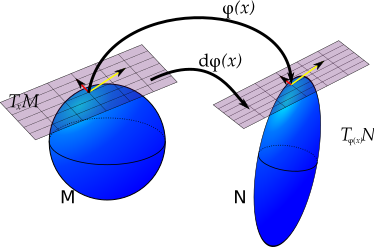
\includegraphics[width=0.5\textwidth]{figures/Pushforward.png}
        \caption{If a map $\phi$, carries every point on manifold \textbf{M} to manifold \textbf{N} then 
        the pushforward of $\phi$ carries vectors in the tangent space at every point in \textbf{M} to a tangent space at every point in \textbf{N}.}
    \end{center}
\end{figure}

In terms of the pushforward map, the \textbf{inverse function theorem} can be stated as follows:
the map \textit{f}: \textbf{M} $\rightarrow$ \textbf{N} is a local diffeomorphism in the neighborhood of a point p 
iff $f_*$ is an isomorphism of T$_p$\textbf{M} and T$_{f(p)}$\textbf{N}.
Thus,we can push vectors forward by any smooth map but you can only push vector
fields forward by a diffeomorphism.

\subsection{Integral Curves and Lie Derivative}
In addition to the exterior derivative of a differential form there is another intrinsic derivative (its definition does not require the introduction of any additional structure) on manifolds. 
If X is a vector field on \textbf{M} then, X can be thought of as a generalized directional derivative operator on functions. 
But to be able to take derivatives of tensor fields, we require pushforward maps since X does not appear to act directly on tensor fields. 

Given a vector field X on \textbf{M}, the fundamental theorem of ODE guarantees that $\exists$ a unique maximal curve $\gamma(t)$: \textbf{I}$\rightarrow$\textbf{M} through
each point p $\epsilon$ \textbf{M} s.t. $\gamma$(0) = p and the tangent vector to the curve $\gamma$ at $\gamma(t)$ is precisely X$_{\gamma(t)}$. 
The curve $\gamma$ is called the \textbf{integral curve} of X through p.

In ordinary calculus, given a curve $\gamma(t)$ (a map to some Euclidean space) $\gamma'(t)$ is naturally a vector (tangent vector to the curve).
But this interpretation is no longer tenable in a general manifold that is not itself a vector space. 
Instead, vectors are derivations, so we really want to understand $\gamma'(t)$ as a derivation.
For this we define \textbf{I} as a manifold (open interval on real line) and attach the coordinate \textit{t} to the points of \textbf{I}. 
Then \textit{d/dt} is a tangent vector field on \textbf{I} which acts on functions \textit{f}: \textbf{I} $\rightarrow \mathbb{R}$ according to \textit{(d/dt)f} = \textit{df/dt}.
Then we can define
\begin{equation}
    \gamma'(t) = \gamma_*(d/dt)_{\gamma(t)}
\end{equation}

This allows us to reduce the question of the existence of an integral curve in a general manifold M to a system of ODEs.
The existence of integral curves enables us to define the notion of a flow. 
At each point p $\epsilon$ \textbf{M} we can imagine moving a parameter a distance \textit{t} along the integral curve $\gamma$ of X through p. 
If we do this for all points of \textbf{M} simultaneously we get a \textbf{flow} along X. 
We can think of this movement as the flow of a fluid as shown in the figure \ref{fig:flow}.
\begin{figure}[ht]
    \begin{center}
        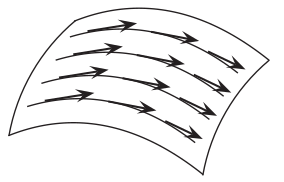
\includegraphics[width=0.4\textwidth]{figures/flow.png}
        \caption{Flowing along the integral curves of a vector field}
        \label{fig:flow}
    \end{center}
\end{figure}

For any open set \textbf{U} of \textbf{M} and any p $\epsilon$ \textbf{U}, define $\gamma_p(t)$ to be the integral curve of X through p, with p = $\gamma_p(0)$. 
Then the map $\phi_t$: \textbf{U} $\rightarrow$ \textbf{M} given by $\gamma_p(0) \rightarrow  \gamma_p(t)$ is a \textbf{flow}, 
or a \textbf{one-parameter group of diffeomorphisms} of \textbf{M} generated by the vector field X. 
Using this flow, we can generalize the notion of the directional derivative to tensor fields.
In terms of flow $\phi_t$,
\begin{equation}
    (Xf)_p =  \lim_{t\to 0} \frac{f_{\phi_t p} - f_p}{t} 
\end{equation}
where $f_p$ = $f(p)$ and $\phi_t p$ = $\gamma_p(t)$

But we cannot do the same with tensors as T$_p$ and T$_{\phi_t p}$ lie on different unrelated vector spaces and thus we cannot subtract them.
However, if we drag T$_{\phi_t p}$ back to p (using pullback) by means of flow $\phi_t$ then we can compare its value with T$_p$. 
So, the right way to define is,
\begin{equation}
    (Xf)_p =  \lim_{t\to 0} \frac{\phi_t^* f - f}{t} \Bigg|_{p}
\end{equation}

By analogy we can define our generalized directional derivative $\mathcal{L}_X$ (\textbf{Lie derivative})
of a tensor field T in the direction X at p by
\begin{equation}
    (\mathcal{L}_X T)_p =  \lim_{t\to 0} \frac{\phi_t^* T - T}{t} \Bigg|_{p} = \frac{d}{dt}\phi_t^* T \Bigg|_{p}
\end{equation}

\textbf{Properties of Lie Derivative:}
\begin{enumerate}
    \itemsep0em
    \item \textbf{preserves tensor type} 
    \item  is \textbf{linear: } $\mathcal{L}_X (S + T)$ = $\mathcal{L}_X S \: T + S \: \mathcal{L}_X T$ 
    \item is a \textbf{derivation: } $\mathcal{L}_X (S \otimes T)$ = $\mathcal{L}_X \otimes S \: T + S \: \mathcal{L}_X\otimes T$
    \item is compatible with the \textbf{natural pairing} of forms and vector fields: 
    $\mathcal{L}_X \langle\omega, Y \rangle$ = $\langle\mathcal{L}_X \omega, Y \rangle$ + $\langle\omega, \mathcal{L}_X Y \rangle$
    \item \textbf{commutation: } For any vector field Y, $\mathcal{L}_X$Y = [X, Y]
    \item For vector fields X, Y, and Z, [$\mathcal{L}_X, \mathcal{L}_Y$]Z = $\mathcal{L}_{[X, Y]}$Z
\end{enumerate}

\newpage
